\section{Pacientes en espera}
En la secciones anteriores se describió la manera de completar el Triage. 

Cada vez que se termina de cargar los síntomas hay dos caminos: ``Fin Triage'' o ``Salir''. Ambas opciones dejan al paciente en una ``Lista de espera'' (figura \ref{fig:espera}).
\begin{figure}
\centerline{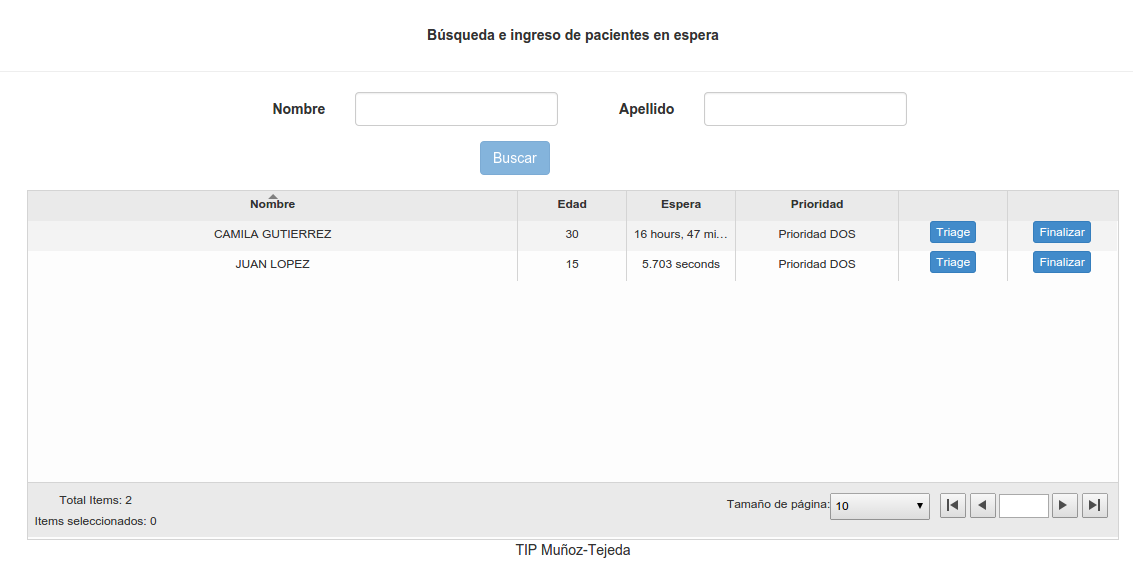
\includegraphics[width=0.99\textwidth]{espera.png}}
\caption{Signos Vitales} \label{fig:espera}
\end{figure}
 La pantalla de lista de espera contiene un cuadro como los vistos anteriormente para la búsqueda de personas así como los filtros para realizar búsquedas en ese cuadro.

Esta pantalla es muy útil cuando la carga de síntomas es realizada por dos personas en ubicaciones físicas distinas. El paciente puede ser atendido en un mostrador (donde se toman sus síntomas, por ejemplo), y luego pasar a un consultorio para la toma de signos vitales. El enfermero en el consultorio debe solamente buscar al paciente en la lista de espera y podrá continuar grabando sus síntomas sin perder ninguna información ya cargada.

\subsubsection{Continuar el Triage}
En el caso de querer continuar el Triage de un paciente en lista de espera, el sistema permite buscar al paciente utilizando el filtro. Una vez localizado, a nivel fila del cuadro encontramos la opción ``Triage'' (figura \ref{fig:espera1})
\begin{figure}
\centerline{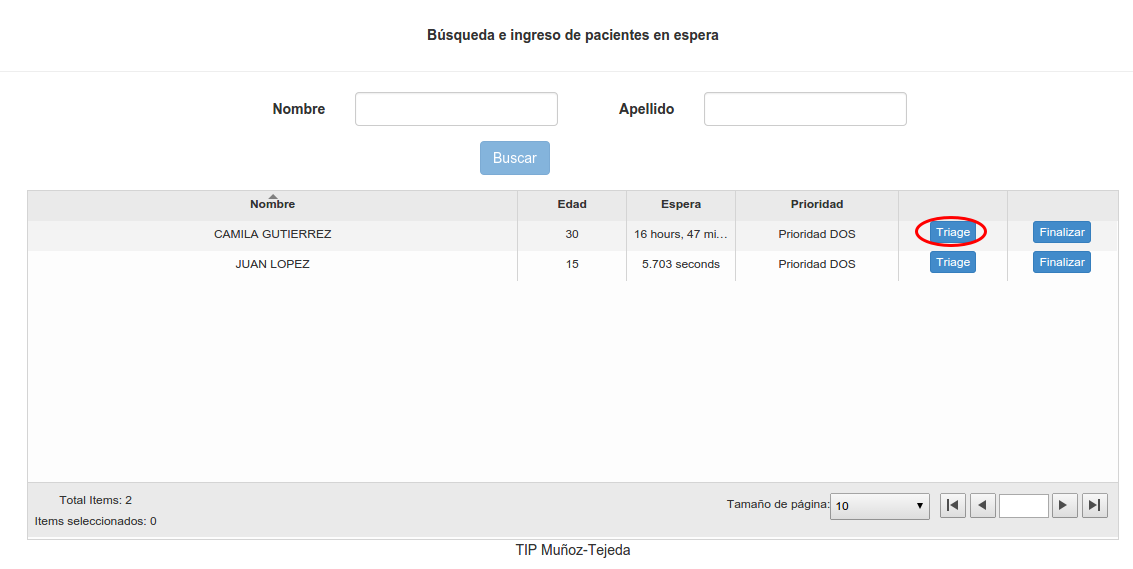
\includegraphics[width=0.99\textwidth]{espera1.png}}
\caption{Signos Vitales} \label{fig:espera1}
\end{figure}
que permite volver a la pantalla de Triage del paciente seleccionado para continuar cargando síntomas.
